
\section{Calculations \& Graphs}

\vspace{-0.5cm}
\singlespacing

%------- Force --------%

\subsection{Final Velocity} 

{\centering
\begin{equation}
	V_f =  \frac{2\Delta{x}}{t} 
	\label{eq:finalV}
\end{equation}
\begin{align*}
	\boldsymbol{\Delta{x}} &: \text{distance between photogates} \\
\boldsymbol{t} &: \text{Average time between photogates} \\
\end{align*}}

\subsubsection{Sample Calculation \\ {\normalfont \small\textit{using measurements of trial 2}}}

{\centering
\begin{align*}
	V_f &=  \frac{2\Delta{x}}{t} \\ \\
			&=  \frac{(2)(0.8744)}{1.456} \\ \\ 
	V_f	&= \boxed{1.201 \text{ m/s}} 
\end{align*}}

%------- ACCELERATION BETWEEN TWO POINTS WITH INITIAL VELOCITY CLOSE TO ZERO--------%

\subsection{Kinetic Energy} 

{\centering
\begin{equation}
	\Delta{\text{KE}} = \frac{1}{2}mv^2 
	\label{eq:energyK}
\end{equation}
\begin{align*}
	\boldsymbol{m} &: \text{mass of glider} \\
	\boldsymbol{v} &: \text{average final velocity of glider} 
\end{align*}}

\subsubsection{Sample Calculation \\ {\normalfont \small\textit{using measurements of trial 2}}}


\begin{align*}
	\Delta{\text{KE}} &= \frac{1}{2}mv^2 \\ \\
										&= \frac{1}{2}(0.2847)(1.201)^2 \\ \\
	\Delta{\text{KE}} &= \boxed{0.2052\,\text{ J}}
\end{align*}

%------- ACCELERATION BETWEEN TWO POINTS --------%

%------- AVERAGE VALUE --------%
\subsection{Gravitational Potential Energy} 

\vspace{0.5cm}

{\centering
\begin{equation}
	\Delta{\text{GPE}} = -mg(\text{h\textsubscript{1}} - \text{h\textsubscript{2}}) 
	\label{eq:energyP}
\end{equation}
\begin{align*}
	\mathbf{m} &: \text{mass of glider}	\\
	\mathbf{g} &: \text{acceleration due to gravity} \\
	\textbf{h\textsubscript{1}} &: \text{height of photogate 1} \\
	\textbf{h\textsubscript{2}} &: \text{height of photogate 2} 
\end{align*}}

\subsubsection{Sample Calculation \\ {\normalfont \small\textit{using measurements of trial 2}}}

\begin{align*}
	\Delta{\text{GPE}} &= -mg(\text{h\textsubscript{1}} - \text{h\textsubscript{2}}) \\
										 &= -(0.2847)(9.80)(0.2346-0.1786) \\
	\Delta{\text{GPE}} &= \boxed{-0.15262\text{ J}}
\end{align*}

\subsection{Average Value Formula} 

\begin{align*}
	\overline{a} = \frac{\text{sum of values}}{\text{total \# of values}} 
\end{align*}

\subsubsection{Sample Calculation \\ {\normalfont \small\textit{using photogate times of trial 2}}}

\begin{align*}
	\overline{a}&=\frac{\text{sum of values}}{\text{total \# of values}} \\ \\
							&= \frac{1.461+1.455+1.454}{3} \\ \\
	\overline{a}&= \boxed{1.457\,\text{s}}
\end{align*}
%------- AVERAGE VALUE --------%

%------- STANDARD DEVIATION --------%
\subsection{Standard Deviation Formula}

\begin{align*}
		\sigma &= \sqrt{\frac{\Sigma(x_i -\overline{a})^2}{N}} \\
		 &= \sqrt{\frac{SS}{N}} \\ \\
		\textbf{N} &:\, \text{Total number of values} \\
		\overline{\textbf{a}} &:\, \text{Average value} \\
		\textbf{x\textsubscript{i}} &:\, \text{Each value from the data set} \\
		\textbf{SS} &:\, \text{Sum of squares} 
\end{align*}

\subsubsection{Sample Calculation \\ {\normalfont \small\textit{std of photogate times with hanging mass at 10 grams }}}

\begin{align*}
	\sigma &= \sqrt{\frac{(1.461-\overline{a})^2 + ... + (1.454-\overline{a})^2}{3}} \\
				 &= \sqrt{\frac{2.886\,\text{x}\,10^{-5}}{3}} \\
		 &= \boxed{0.0003\, \text{s}}
\end{align*}
%------- STANDARD DEVIATION --------%

%------- RELATIVE ERROR --------%
\subsection{Percent Difference Between Change in KE and GPE}
\vspace{0.5cm}
\begin{equation}
	PD = \left| {\frac{\frac{\Delta{\textbf{KE}} + \Delta{\text{GPE}}}{\Delta{\text{KE}} - \Delta{\text{GPE}}}}{2}} \right|\: \text{x}\: 100\% \\ \\
	\label{eq:pdiff}
\end{equation}
\begin{align*}
	\boldsymbol{\Delta{\textbf{KE}}} &:\, \text{Change in kinetic energy of glider} \\
	\boldsymbol{\Delta{\textbf{GPE}}} &:\, \text{Change in gravitational energy of glider} 
\end{align*}

\subsubsection{Sample Calculation \\ {\normalfont \small\textit{using measurements from trial 2}}}

\begin{align*}
	PD &= \left| {\frac{\frac{\Delta{\textbf{KE}} + \Delta{\text{GPE}}}{\Delta{\text{KE}} - \Delta{\text{GPE}}}}{2}} \right|\: \text{x}\: 100\% \\
	 &= \left| {\frac{\frac{0.2502 + (-0.1562}{0.2052 - (-0.1562)}}{2}} \right|\: \text{x}\: 100\% \\
			PD &= \boxed{27.12\%} 
\end{align*}
%------- RELATIVE ERROR --------%

%----TABLES-----%
\begin{landscape}
\begin{table}
\centering
\captionsetup{font=Large}
\caption{Energy Loss of Glider Trials}
\label{tab:dataTab}
\resizebox{\linewidth}{!}{%
\begin{tabular}{lr|lr|lr} 
\hline
\multicolumn{2}{c|}{\textbf{TRIAL 1}}                                                 & \multicolumn{2}{c|}{\textbf{TRIAL 2}}                                                 & \multicolumn{2}{c}{\textbf{TRIAL 3}}                                                  \\ 
\hline
\textbf{m (kg)}                                              & 0.1847                 & \textbf{m (kg)}                                              & 0.2847                  & \textbf{m (kg)}                                              & 0.3847                  \\
                                                             & \multicolumn{1}{l|}{~} & ~                                                            & \multicolumn{1}{l|}{~} &                                                              & \multicolumn{1}{l}{}   \\
$\mathbf{x_2\textbf{ (m)}}$                                  & 1.572                  & $\mathbf{x_2\textbf{ (m)}}$                                  & 0.4016                 & $\mathbf{x_2\textbf{ (m)}}$                                  & 0.4016                 \\
$\mathbf{x_1\textbf{ (m)}}$                                  & 0.3883                 & $\mathbf{x_1\textbf{ (m)}}$                                  & 1.276                  & $\mathbf{x_1\textbf{ (m)}}$                                  & 1.276                  \\
$\mathbf{\Delta{x}\textbf{ (m)}}$                             & 1.1840                 & $\mathbf{\Delta{x}\textbf{ (m)}}$                             & 0.8744                 & $\mathbf{\Delta{x}\textbf{ (m)}}$                             & 0.8744                 \\
                                                             & \multicolumn{1}{l|}{~} & ~                                                            & \multicolumn{1}{l|}{~} &                                                              & \multicolumn{1}{l}{}   \\
$\mathbf{h_2\textbf{ (m)}}$                                  & 0.2555                 & $\mathbf{h_2\textbf{ (m)}}$                                  & 0.1786                 & $\mathbf{h_2\textbf{ (m)}}$                                  & 0.1786                 \\
$\mathbf{h_1\textbf{ (m)}}$                                  & 0.1786                 & $\mathbf{h_1\textbf{ (m)}}$                                  & 0.2346                 & $\mathbf{h_1\textbf{ (m)}}$                                  & 0.2346                 \\
$\mathbf{\Delta{h}\textbf{ (m)}}$                             & 0.0769                 & $\mathbf{\Delta{h}\textbf{ (m)}}$                             & 0.0560                 & $\mathbf{\Delta{h}\textbf{ (m)}}$                             & 0.0560                 \\
                                                             & \multicolumn{1}{l|}{~} & ~                                                            & \multicolumn{1}{l|}{~} &                                                              & \multicolumn{1}{l}{}   \\
$\mathbf{t_1\textbf{ (s)}}$                                  & 1.648                  & $\mathbf{t_1\textbf{ (s)}}$                                  & 1.461                  & $\mathbf{t_1\textbf{ (s)}}$                                  & 1.458                  \\
$\mathbf{t_2\textbf{ (s)}}$                                  & 1.686                  & $\mathbf{t_2\textbf{ (s)}}$                                  & 1.455                  & $\mathbf{t_2\textbf{ (s)}}$                                  & 1.424                  \\
$\mathbf{t_3\textbf{ (s)}}$                                  & 1.656                  & $\mathbf{t_3\textbf{ (s)}}$                                  & 1.454                  & $\mathbf{t_3\textbf{ (s)}}$                                  & 1.454                  \\
$\mathbf{t_\textbf{std} \textbf{ (s)}}$                      & 0.016                  & $\mathbf{t_\textbf{std} \textbf{ (s)}}$                      & 0.003                  & $\mathbf{t_\textbf{std} \textbf{ (s)}}$                      & 0.015                  \\
$\mathbf{t_\textbf{avg} \textbf{ (s)}}$                      & 1.663                  & $\mathbf{t_\textbf{avg} \textbf{ (s)}}$                      & 1.457                  & $\mathbf{t_\textbf{avg} \textbf{ (s)}}$                      & 1.446                  \\
                                                             & \multicolumn{1}{l|}{~} & ~                                                            & \multicolumn{1}{l|}{~} &                                                              & \multicolumn{1}{l}{}   \\
$\mathbf{V_f\textbf{avg}\textbf{ (m/s)}}$ & 1.424                  & $\mathbf{V_f\textbf{avg}\textbf{ (m/s)}}$ & 1.201                  & $\mathbf{V_f\textbf{avg}\textbf{ (m/s)}}$ & 1.21                   \\
$\mathbf{\Delta{\textbf{KE}_\textbf{avg}} \textbf{ (J)}}$    & 0.1871                  & $\mathbf{\Delta{\textbf{KE}_\textbf{avg}} \textbf{ (J)}}$    & 0.2052                  & $\mathbf{\Delta{\textbf{KE}_\textbf{avg}} \textbf{ (J)}}$    & 0.2815                  \\
$\mathbf{\Delta{\textbf{GPE}_\textbf{avg}} \textbf{ (J)}}$   & -0.1392                 & $\mathbf{\Delta{\textbf{GPE}_\textbf{avg}} \textbf{ (J)}}$   & -0.1562                 & $\mathbf{\Delta{\textbf{GPE}_\textbf{avg}} \textbf{ (J)}}$   & -0.2111                 \\
~                                                            & \multicolumn{1}{l|}{~} & ~                                                            & \multicolumn{1}{l|}{~} & ~                                                            & \multicolumn{1}{l}{~}  \\ 
\hline
\textbf{Percent Difference (\%)}                             & 29.36                  & \textbf{Percent Difference (\%)}                             & 27.12                  & \textbf{Percent Difference (\%)}                             & 28.58                  \\
\textbf{Energy Lost (J)}                                     & 0.04796                  & \textbf{Energy Lost (J)}                                     & 0.04897                  & \textbf{Energy Lost (J)}                                     & 0.0704                   \\
\hline
\end{tabular}
}
\end{table}
\end{landscape}
%----TABLES-----%

%----GRAPHS-----%

% \begin{landscape}
% \subsection{Graphs}
% \begin{figure}[H]
% 	\begin{center}
% 		\captionsetup{font=Large}
% 		\caption{Force vs. Acceleration}\label{fig:GFvA}
% 		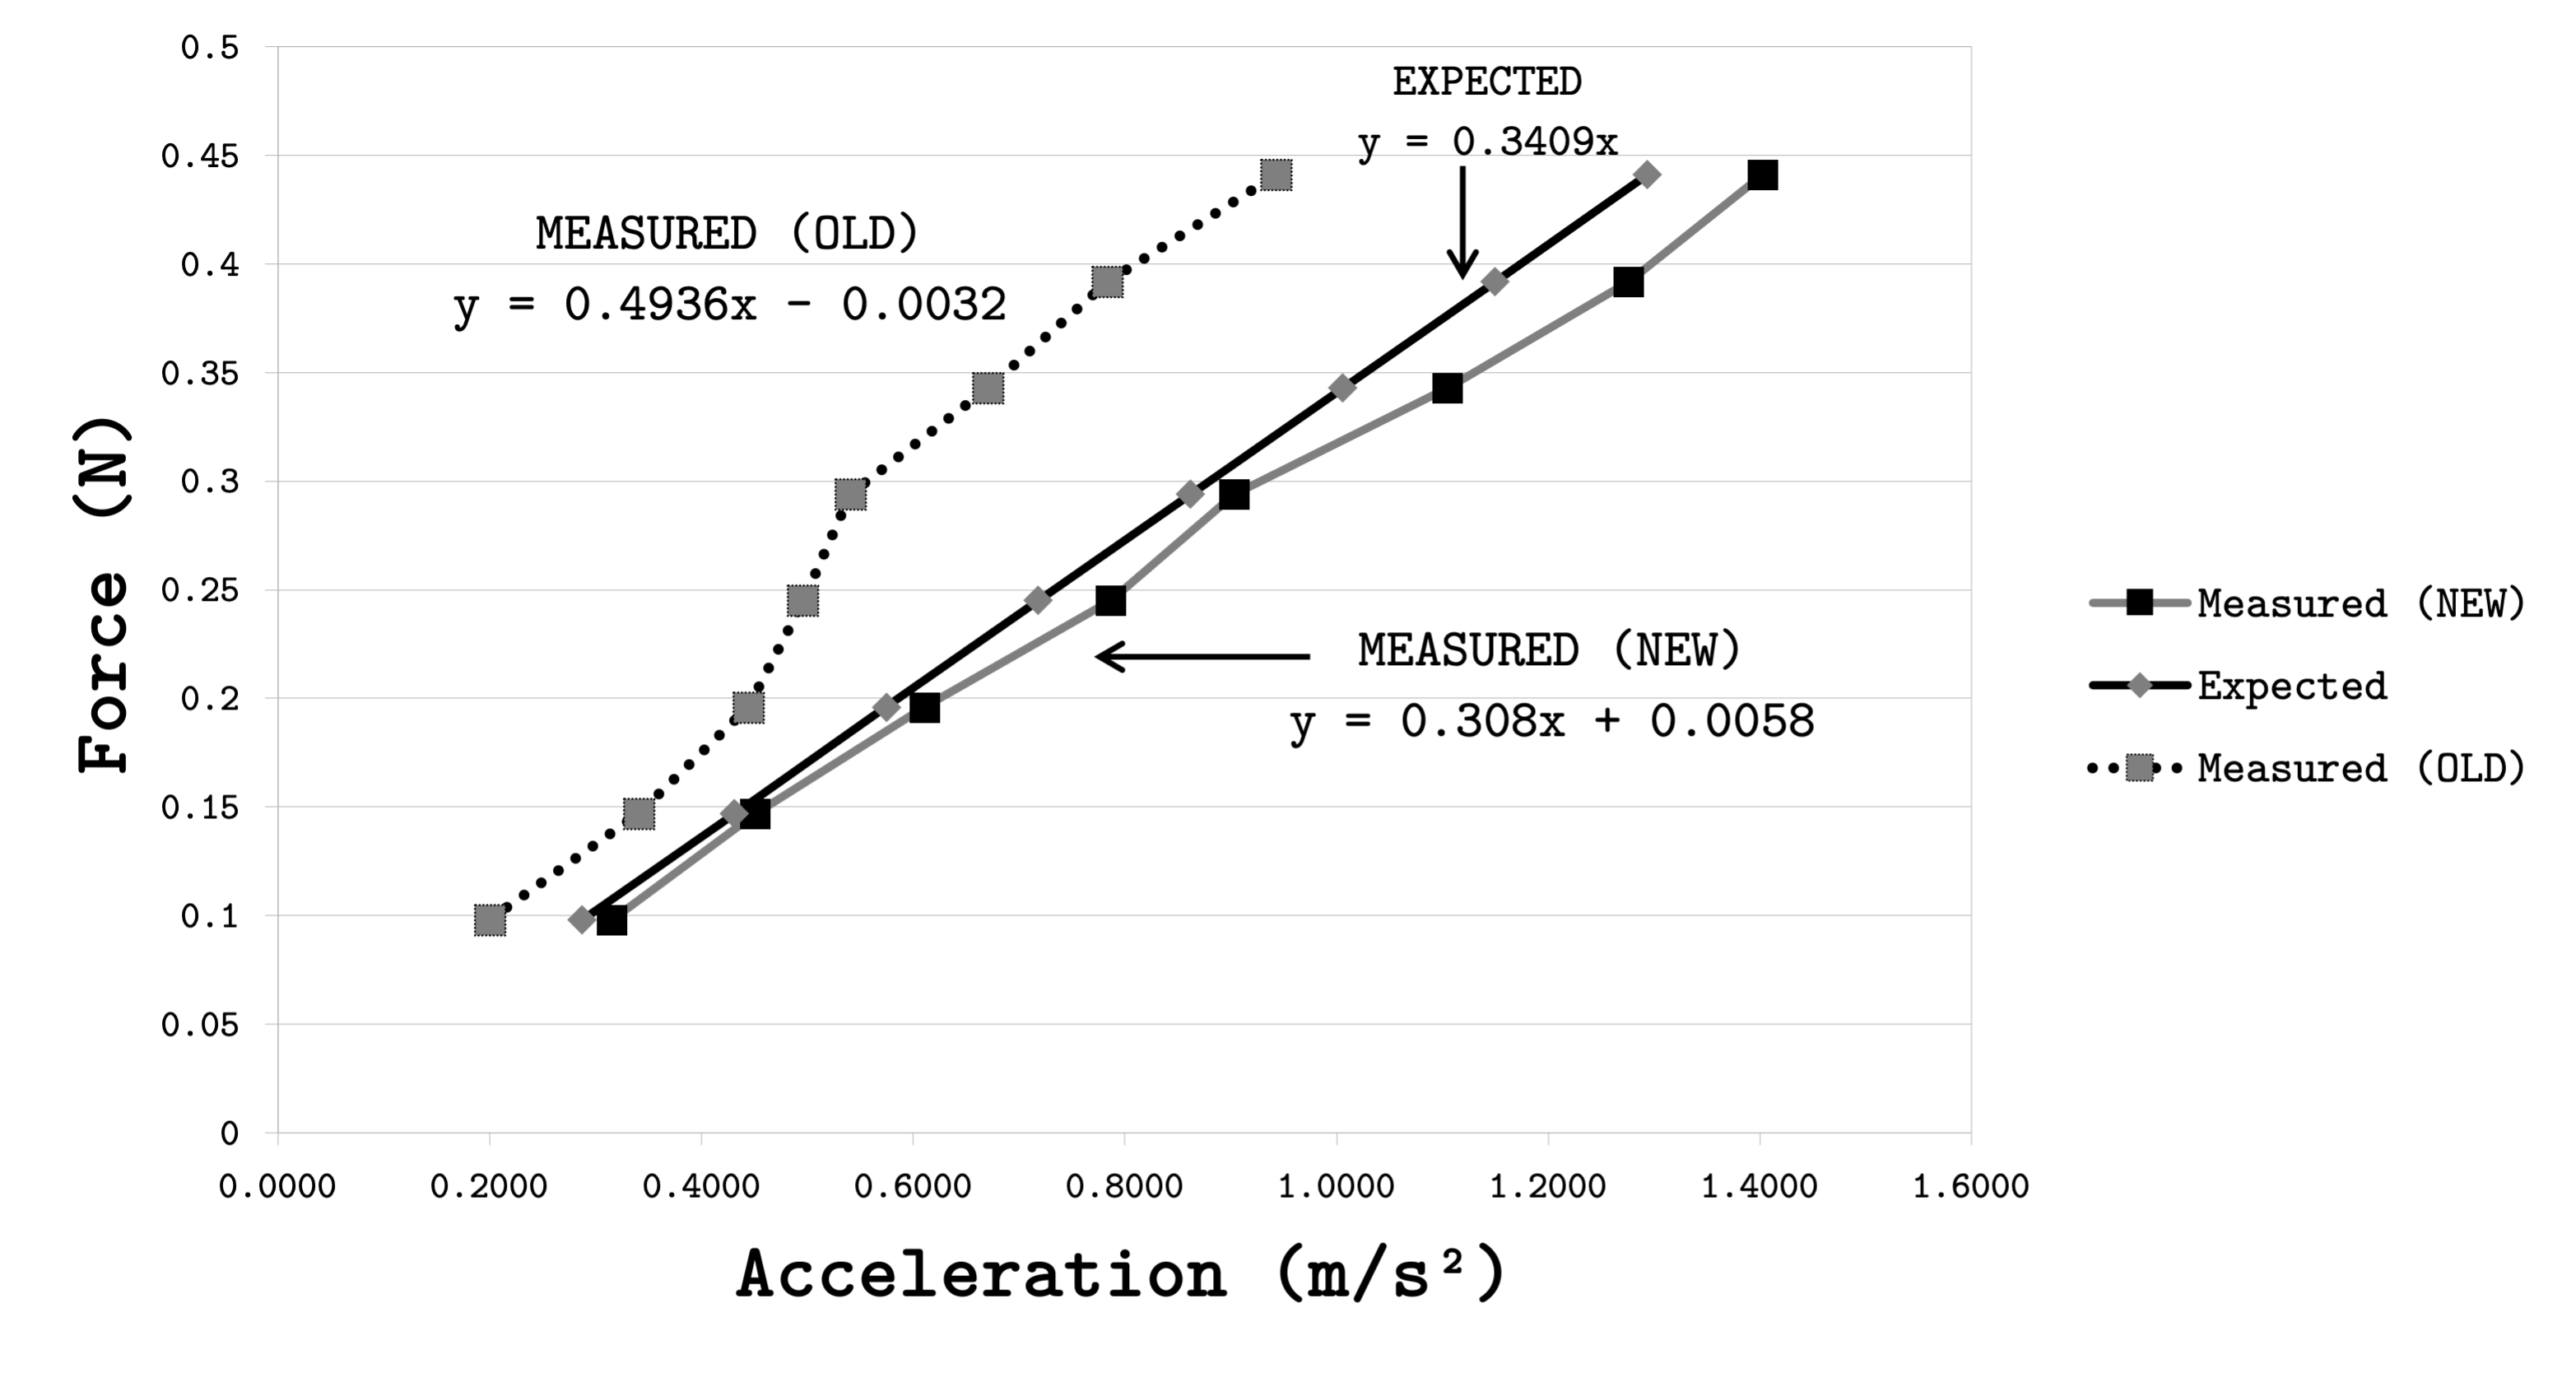
\includegraphics[width=0.90\columnwidth]{images/GraphFvA}
% 	\end{center}
% \end{figure}
% \end{landscape}

%----GRAPHS-----%

\newpage

